\RequirePackage{luatex85}
\documentclass[tikz]{standalone}

\usetikzlibrary{arrows,calc,fit,positioning,backgrounds}

\usepackage{fontspec}
\setmainfont{Source Sans Pro}

\tikzset{
  >=latex,
  every path/.style={
    shorten <=2pt,shorten >=2pt,>=stealth
  },
  background rectangle/.style={fill=white},
  note/.style={
    font=\scriptsize
  },
  component/.style={
    rectangle,rounded corners,draw=black,
    text depth=0pt,
    minimum width=4cm,
    minimum height=8mm
  },
  small component/.style={
    component,
    text depth=0pt,
    font=\footnotesize,
    minimum width=20mm,
    minimum height=6mm,
  },
  dag/.style={
    component,draw=gray,line width=2pt,
    inner sep=3mm,
  },
  daglabel/.style={
    fill=white,
    text depth=0pt,
    font=\footnotesize,
    minimum height=6mm
  },
  prejob/.style={
    draw,
    minimum width=16mm,
    minimum height=6mm,
    text depth=0pt,
    font=\footnotesize,
    % append after command={
    %   \pgfextra
    %   \draw[shorten <=0pt, shorten >=0pt,black,rounded corners]%
    %   (\tikzlastnode.south east)%
    %     -- (\tikzlastnode.south)%
    %     -| (\tikzlastnode.west)%
    %     |- (\tikzlastnode.north)%
    %     -- (\tikzlastnode.north east);
    %   \endpgfextra
    % }
  },
  postjob/.style={
    draw,
    minimum width=16mm,
    minimum height=6mm,
    text depth=0pt,
    font=\footnotesize,
    % append after command={
    %   \pgfextra
    %   \draw[shorten <=0pt, shorten >=0pt,black,rounded corners]%
    %   (\tikzlastnode.north west)%
    %     -- (\tikzlastnode.north)%
    %     -| (\tikzlastnode.east)%
    %     |- (\tikzlastnode.south)%
    %     -- (\tikzlastnode.south west);
    %   \endpgfextra
    % }
  },
  mainjob/.style={
    component,
    rounded corners=0,
    minimum height=6mm,
    minimum width=25mm,
    text depth=0pt,
    font=\footnotesize,
  },
  optional/.style={
    dashed
  }
}


\begin{document}

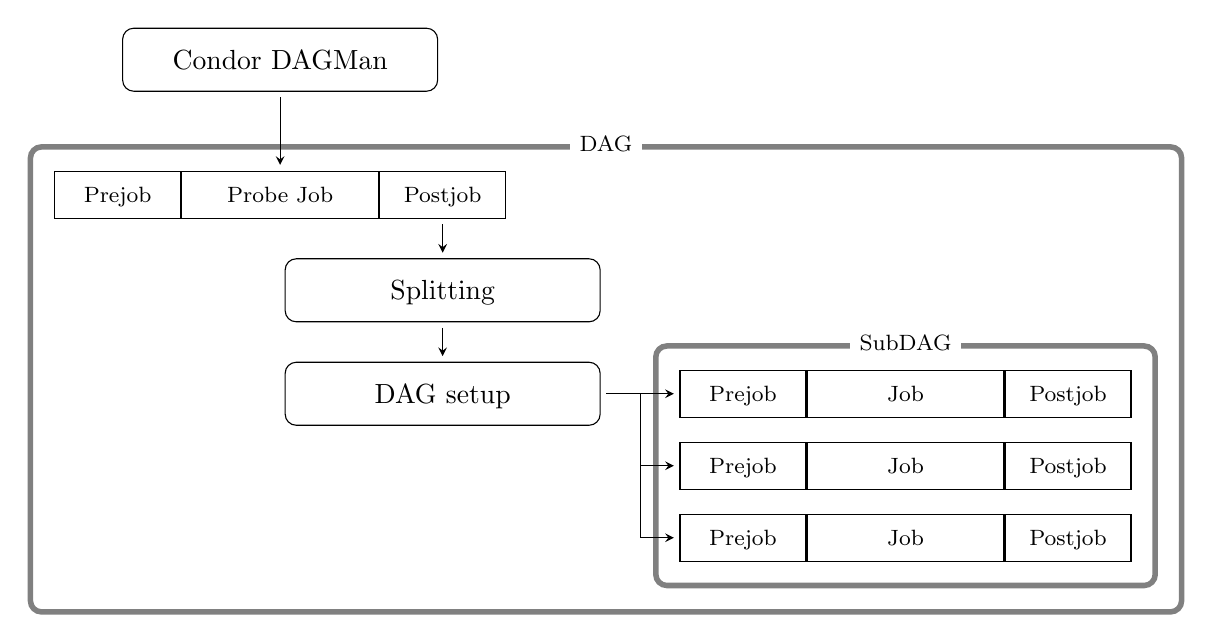
\begin{tikzpicture}
  \node[component] (dagm) {Condor DAGMan};

  \node[mainjob,below=of dagm] (probe-job) {Probe Job};
  \node[prejob,anchor=east] (probe-pre) at (probe-job.west) {Prejob};
  \node[postjob,anchor=west] (probe-post) at (probe-job.east) {Postjob};

  \node[component,below=5mm of probe-post] (split) {Splitting};
  \node[component,below=5mm of split] (creat) {DAG setup};

  \node[prejob,right=of creat] (pre) {Prejob};
  \node[mainjob,anchor=west] (job) at (pre.east) {Job};
  \node[postjob,anchor=west] (post) at (job.east) {Postjob};

  \node[prejob,below=3mm of pre] (pre2) {Prejob};
  \node[mainjob,anchor=west] (job2) at (pre2.east) {Job};
  \node[postjob,anchor=west] (post2) at (job2.east) {Postjob};

  \node[prejob,below=3mm of pre2] (pre3) {Prejob};
  \node[mainjob,anchor=west] (job3) at (pre3.east) {Job};
  \node[postjob,anchor=west] (post3) at (job3.east) {Postjob};

  \node[dag,fit=(pre) (post3)] (subdag) {};
  \node[daglabel] at (subdag.north) {SubDAG};

  \node[dag,fit=(probe-pre) (subdag)] (dag) {};
  \node[daglabel] at (dag.north) {DAG};

  % Flow
  \draw[->] (dagm) -- (probe-job);
  \draw[->] (probe-post) -- (split);
  \draw[->] (split) -- (creat);
  \draw[->] (creat) -- (pre);
  \draw[shorten <=0,->] ($(creat.east)!.5!(pre.west)$) |- (pre2);
  \draw[shorten <=0,->] ($(creat.east)!.5!(pre.west)$) |- (pre3);
\end{tikzpicture}

\end{document}
